%%%%%%%%%%%%%%%%%%%%%%%%%
% !TEX TS-program = pdflatex
% !TEX root = ../tesis.tex
%%%%%%%%%%%%%%%%%%%%%%
%% CHAPTER 1
%%%%%%%%%%%%%%%%%%%%%%

\chapter{Introduction}\label{chap_01}
%%%%%%%%%%%%%%%%%%%%%%%%%
\minitoc
%\clearpage

\section{Motivation}\label{sec_motivation}

This template has been created specifically for the defence of Thesis~\cite{tesis}. If you make use of this template or base your work on it, please provide proper attribution or reference to its original source.



\section{Aims and objectives}\label{sec_aims}

This template uses the \texttt{acronym} package to manage abbreviations consistently throughout the text. Acronyms should be defined inside the \texttt{acronym} environment and referenced in the text using dedicated commands. The usage is summarised below:

\begin{itemize}
    \item \verb|\ac{cd}| — On first use, prints the full name followed by the acronym in parentheses: \ac{CNN}. Later uses show only the acronym: \ac{CNN}.
    
    \item \verb|\acs{cd}| — Prints only the short form (the acronym), even on first use: \acs{AD}.
    
    \item \verb|\acl{cd}| — Prints only the long form (the full name): \acl{CNN}.
    
    \item \verb|\acf{cd}| — Always prints the full name and acronym: \acf{AD}.
    
    \item \verb|\acp{cd}| — Prints the plural form, automatically adding an “s” to the acronym and adjusting the long form if defined: \acp{CNN}.
\end{itemize}

All acronyms must be defined in the \texttt{acronym} environment.


\section{Organisation of this thesis}\label{sec_organization}

This thesis is organised... It is divided into various topics and chapters as illustrated in Figure~\ref{fig:01_objetivos}.

\begin{figure*}[htbp]
\centering
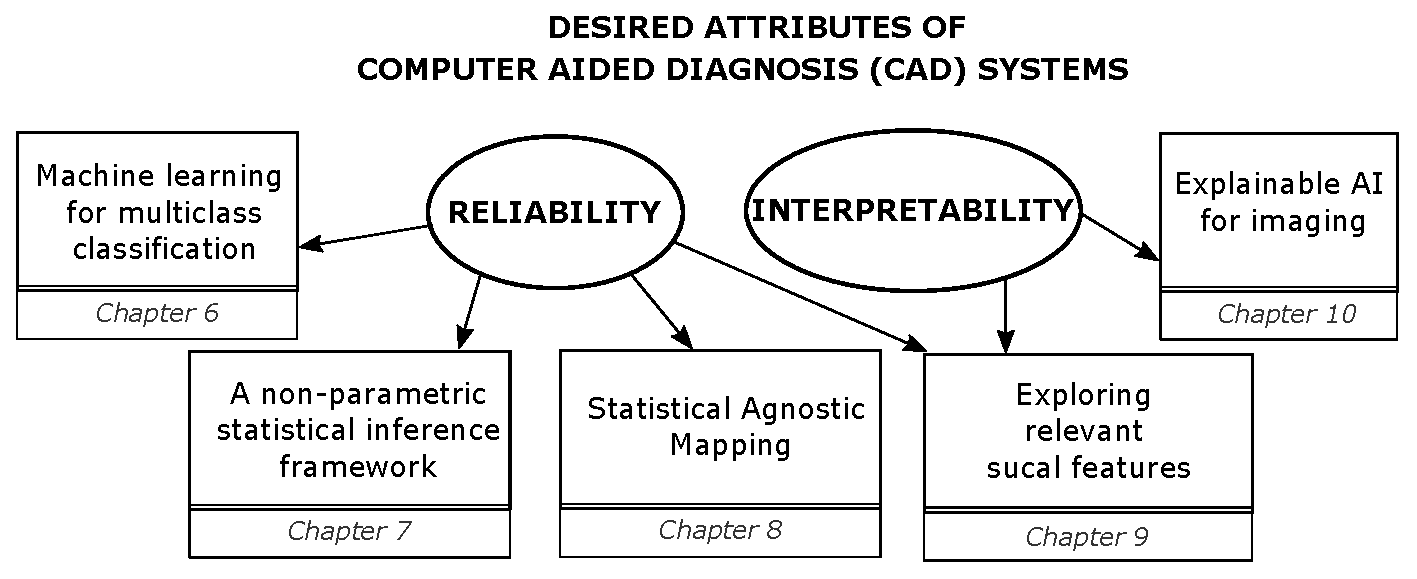
\includegraphics[width=0.8\textwidth]{Figures/chap_01/objetivos}
\caption{Structured scheme of the content of the contributions of this thesis. }
\label{fig:01_objetivos}
\end{figure*}


\section{Contributions}\label{sec_controbutions}

Part of the content of this thesis, including figures and tables, has been published in several international journal articles and conference presentations. These contributions are detailed below.

\subsection*{Articles}

\bibentry{JimenezMesa2020} (\textbf{chapter~\ref{chap_04}})


\subsection*{Conferences}

\bibentry{JimenezMesa2020} (\textbf{chapter~\ref{chap_04}})




